\section*{Gennemgang af det orginal program}
Dette vil være en gennemgang af det orginale program, og nogle tal på performance.

Der var ingen måder i programmet at måle på sig selv, så der er blevet introduceret en ny klasse, til at kunne fortage målinger.




\lstset{ %
language=Java,                % choose the language of the code
basicstyle=\footnotesize,       % the size of the fonts that are used for the code
numbers=left,                   % where to put the line-numbers
numberstyle=\footnotesize,      % the size of the fonts that are used for the line-numbers
stepnumber=1,                   % the step between two line-numbers. If it is 1 each line will be numbered
numbersep=5pt,                  % how far the line-numbers are from the code
backgroundcolor=\color{white},  % choose the background color. You must add \usepackage{color}
showspaces=false,               % show spaces adding particular underscores
showstringspaces=false,         % underline spaces within strings
showtabs=false,                 % show tabs within strings adding particular underscores
frame=single,           % adds a frame around the code
tabsize=2,          % sets default tabsize to 2 spaces
captionpos=b,           % sets the caption-position to bottom
breaklines=true,        % sets automatic line breaking
breakatwhitespace=false,    % sets if automatic breaks should only happen at whitespace
escapeinside={\%*}{*)}          % if you want to add a comment within your code
}

\begin{lstlisting}
public class Timer {
    private long start, spent = 0;
    private double st= 0.0,sst=0.0;
    int n = 0;
    public Timer() { play(); }
    public double check() {
        double time = (System.nanoTime() - start+spent);
        st += time;
        sst += time * time ;
        n++;
        return (System.nanoTime() - start+spent)/1e6;
    }
    public void play() { start = System.nanoTime(); }
    public double getMean(){
        return (st/n)/1e6;
    }
    public double getSDev(){
        return (Math.sqrt((sst -getRealMean()*getRealMean()-n)/(n-1)))/1e6;
    }
    private double getRealMean(){
        return st/n;
    }
}
\end{lstlisting}

Denne klasse kan returnere tiden i milliesekunder fra play() til check().
Den kan også returnere empirical mean med getMean() og standard deviation med getSDev().

\subsection*{performance}
Med klassen fra sidste kapitel, er der fortaget målinger af det orginale program.


De første målinger er taget ved at køre programmet 50 gange og tage en måling fra hver gang.


\begin{lstlisting}
113 ms
73 ms
80 ms
84 ms
68 ms
42 ms
42 ms
40 ms
44 ms
46 ms
50 ms
43 ms
48 ms
45 ms
44 ms
41 ms
53 ms
38 ms
39 ms
40 ms
39 ms
39 ms
41 ms
39 ms
38 ms
39 ms
43 ms
71 ms
65 ms
40 ms
38 ms
79 ms
59 ms
38 ms
38 ms
40 ms
38 ms
37 ms
38 ms
39 ms
40 ms
38 ms
38 ms
40 ms
43 ms
41 ms
38 ms
39 ms
38 ms
40 ms
\end{lstlisting}

Dette er sat i en boksplot for at give et intryk af programmets performancen.
\begin{figure}
  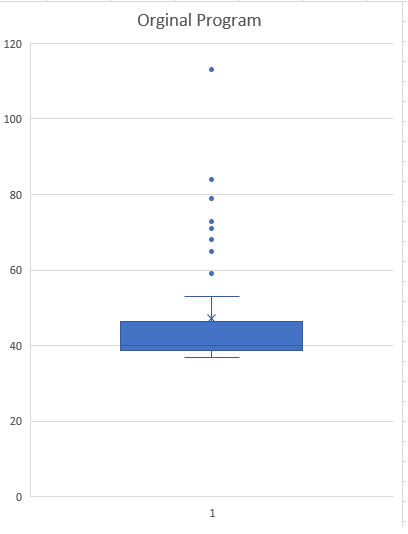
\includegraphics[width=0.4\linewidth]{orginalboks.png}
  \caption{Boksplot af det orginale program}
  \label{fig:orginal}
\end{figure}
\newpage
Dernæste er de 50 gange blevet kørt 50 gange for at skabe mean og standard deviation.
så hver linie i følgnede er 50 kørsler af programmet.

\begin{lstlisting}
mean is : 45,04 MS +/-  47,17 MS
mean is : 41,95 MS +/-  43,24 MS
mean is : 40,82 MS +/-  41,75 MS
mean is : 40,50 MS +/-  41,26 MS
mean is : 40,09 MS +/-  40,71 MS
mean is : 39,86 MS +/-  40,39 MS
mean is : 39,67 MS +/-  40,13 MS
mean is : 39,57 MS +/-  40,01 MS
mean is : 39,44 MS +/-  39,84 MS
mean is : 39,35 MS +/-  39,72 MS
mean is : 39,26 MS +/-  39,60 MS
mean is : 39,26 MS +/-  39,59 MS
mean is : 39,24 MS +/-  39,55 MS
mean is : 39,22 MS +/-  39,53 MS
mean is : 39,15 MS +/-  39,44 MS
mean is : 39,12 MS +/-  39,39 MS
mean is : 39,18 MS +/-  39,48 MS
mean is : 39,15 MS +/-  39,43 MS
mean is : 39,16 MS +/-  39,44 MS
mean is : 39,21 MS +/-  39,49 MS
mean is : 39,19 MS +/-  39,46 MS
mean is : 39,18 MS +/-  39,45 MS
mean is : 39,18 MS +/-  39,44 MS
mean is : 39,25 MS +/-  39,51 MS
mean is : 39,21 MS +/-  39,46 MS
mean is : 39,19 MS +/-  39,43 MS
mean is : 39,21 MS +/-  39,45 MS
mean is : 39,20 MS +/-  39,43 MS
mean is : 39,19 MS +/-  39,41 MS
mean is : 39,18 MS +/-  39,40 MS
mean is : 39,16 MS +/-  39,38 MS
mean is : 39,16 MS +/-  39,37 MS
mean is : 39,19 MS +/-  39,39 MS
mean is : 39,19 MS +/-  39,40 MS
mean is : 39,22 MS +/-  39,42 MS
mean is : 39,23 MS +/-  39,43 MS
mean is : 39,21 MS +/-  39,41 MS
mean is : 39,23 MS +/-  39,43 MS
mean is : 39,23 MS +/-  39,42 MS
mean is : 39,25 MS +/-  39,44 MS
mean is : 39,24 MS +/-  39,44 MS
mean is : 39,23 MS +/-  39,41 MS
mean is : 39,23 MS +/-  39,42 MS
mean is : 39,21 MS +/-  39,40 MS
mean is : 39,21 MS +/-  39,39 MS
mean is : 39,21 MS +/-  39,39 MS
mean is : 39,20 MS +/-  39,38 MS
mean is : 39,20 MS +/-  39,38 MS
mean is : 39,20 MS +/-  39,37 MS
mean is : 39,20 MS +/-  39,37 MS
\end{lstlisting}


\subsection*{Flaskehalsen}
For at finde flaskehalsen i programmet, er der startet i main, og tids målingen er flyttet rundt til at finde det præcise sted hvor tiden bliver brugt.

\begin{lstlisting}
Timer t = new Timer();
                String fileName = "src/main/resources/FoundationSeries.txt";
                Reader reader = new FileReader(fileName);
                Map<Integer, Long> freq = new HashMap<>();
                t.play();
                tallyChars(reader, freq);
                timeSets[x] = t.check();
                print_tally(freq);
\end{lstlisting}

Da tidsmålingen målte på tallyChars(), viste målingen at det var her, 99% af tiden blev brugt. Og en optimerings løsning var i denne funktion.



